\documentclass{standalone}

\usepackage{pgf,tikz}
\usepackage{mathrsfs}
\usetikzlibrary{arrows}
\pagestyle{empty}
\begin{document}

	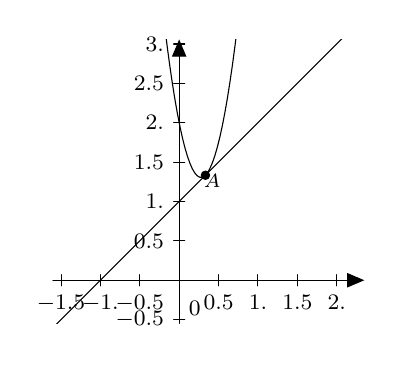
\begin{tikzpicture}[line cap=round,line join=round,>=triangle 45,x=1.0cm,y=1.0cm]
	\draw[->,color=black] (-1.6028511446403986,0.) -- (2.3511905834337297,0.);
	\foreach \x in {-1.5,-1.,-0.5,0.5,1.,1.5,2.}
	\draw[shift={(\x,0)},color=black] (0pt,2pt) -- (0pt,-2pt) node[below] {\footnotesize $\x$};
	\draw[->,color=black] (0.,-0.5470600513062651) -- (0.,3.0578861007757325);
	\foreach \y in {-0.5,0.5,1.,1.5,2.,2.5,3.}
	\draw[shift={(0,\y)},color=black] (2pt,0pt) -- (-2pt,0pt) node[left] {\footnotesize $\y$};
	\draw[color=black] (0pt,-10pt) node[right] {\footnotesize $0$};
	\clip(-1.6028511446403986,-0.5470600513062651) rectangle (2.3511905834337297,3.0578861007757325);
	\draw [samples=50,rotate around={0.:(0.2777777777777778,1.3055555555555556)},xshift=0.2777777777777778cm,yshift=1.3055555555555556cm,domain=-0.7777777777777777:0.7777777777777777)] plot (\x,{(\x)^2/2/0.05555555555555555});
	\draw [domain=-1.6028511446403986:2.3511905834337297] plot(\x,{(--1.--1.*\x)/1.});
	\begin{scriptsize}
	\draw [fill=black] (0.3333333333333333,1.3333333333333333) circle (1.5pt);
	\draw[color=black] (0.4204783162119482,1.2625374242447773) node {$A$};
	\end{scriptsize}
	\end{tikzpicture}
\end{document}